\section{Performance Evaluation}
\subsection{Simulation Settings}
\subsection{Performance Comparison}


\begin{frame}
	\frametitle{Simulation Settings}
	
	\begin{table}
		\renewcommand{\arraystretch}{1.2}
		\captionsetup{name=TABLE}
		%\caption{Simulation Parameters}
		\scalebox{0.7}{%
			\begin{tabular}{ l|l } 
				\toprule
				\textbf{Parameter} & \textbf{Value}  \\ 
				\midrule
				%Number of MDs $i$  & 50  \\ 
				%Number of EN $j$  & 5  \\ 
				%Number of episodes $\textit{Ep.}$  & 1000  \\ 
				%Number of time slots $T$  & 100 (with $\tau = 0.1$ second) \\ 
				Computation capacity of MD $f_i$  & 2.6 GHz \\ 
				Computation capacity of EN $f_j^{\text{E}}$ & 42.8 GHz  \\ 
				Transmission capacity of MD $r_{i,j}(t)$ & 14 Mbps  \\ 
				Task arrival rate & 150 Task/Sec  \\ 
				Size of task $\lambda_i(t)$  & $\{\text{1.0, 1.1, \ldots , 7.0}\}$ Mbits \\ 
				Required CPU cycles of task $\rho_i(t)$  & $\{\text{0.197,0.297,0.397}\}$G/Mbits \\ 
				Deadline of task $ \Delta_i$  & 10 time slots (1 Sec)\\ 
				Battery level of MD $\phi_i(t)$  & $\{\text{25, 50, 75}\}$ Percent \\ 
				Computation power of MD $p_i^{\text{C}}$ & \text{$10^{-27}(f_i)^3$}  \\ 
				Computation power of EN $p_j^{\text{E}}$ & 5 w  \\ 
				Transmission power of MD $p_i^{\text{T}}$ & 2.3 w  \\ 
				Standby power of MD $p_i^{\text{I}}$& 0.1 w  \\ 
		\end{tabular}}
		\label{table}
	\end{table}


	\vfill

 50 MD	and   5 EN  \\ 
 1000 Episode and 100 Time Slot 

\end{frame}

\begin{frame}
	\frametitle{Performance Comparison}
	
	\textbf{Benchmark Methods:}
			\vspace{4mm}
	
	\begin{itemize}[]
		
		\item \textcolor{teal}{Local Computing (LC)}:  MDs execute all of their computation tasks using their own computing capacity 
					\vspace{2mm}
		\item \textcolor{teal}{Full Offloading (FO)}: MDs dispatches all of their computation tasks to ENs and selects their offloading target randomly
					\vspace{2mm}
		\item \textcolor{teal}{Random Decision (RD)}: MDs randomly makes offloading decisions and selects the offloading target 
					\vspace{2mm}
		\item \textcolor{teal}{PGOA}[21]: A distributed optimization algorithm designed for delay-sensitive tasks in an environment where MDs interact strategically with multiple ENs.
		
	\end{itemize}
	
\end{frame}

\begin{frame}
	\frametitle{Performance Comparison}

 \begin{figure}
	%\captionsetup{name=Fig.}
	\begin{minipage}[b]{0.47\linewidth}
		\centering
		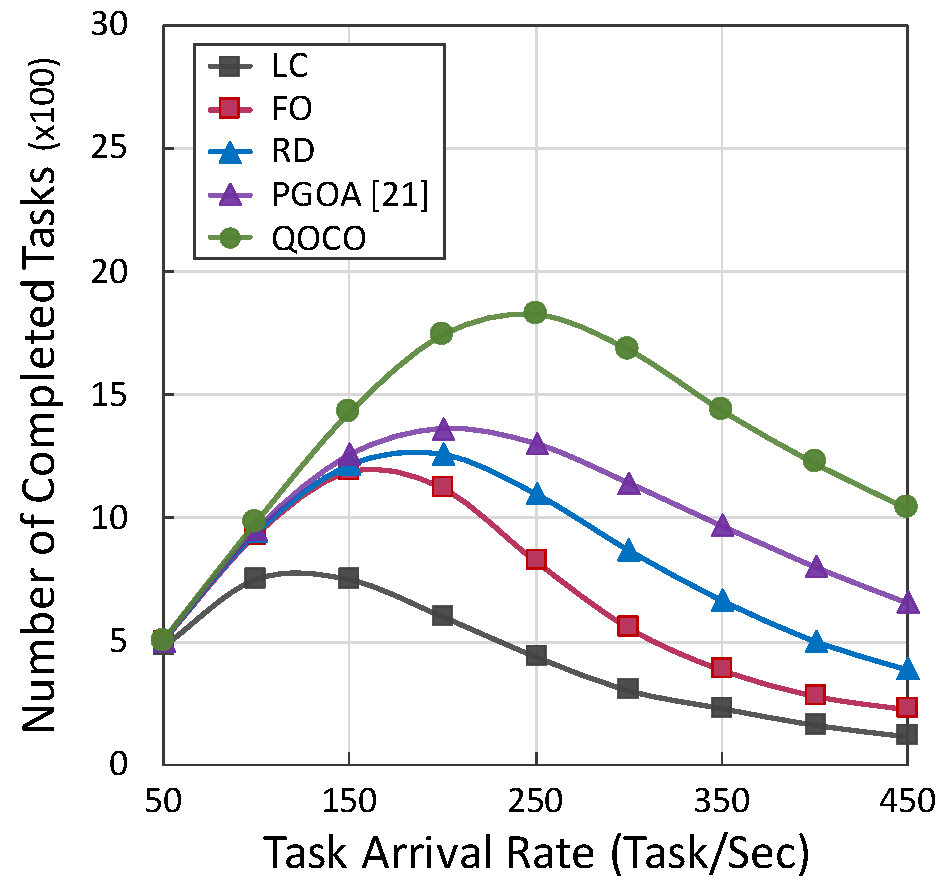
\includegraphics[width=\textwidth]{111} 
       \hspace{0.6cm}(a)
	\end{minipage}
	\hspace{-0.2cm}
	\begin{minipage}[b]{0.47\linewidth}
		\centering
		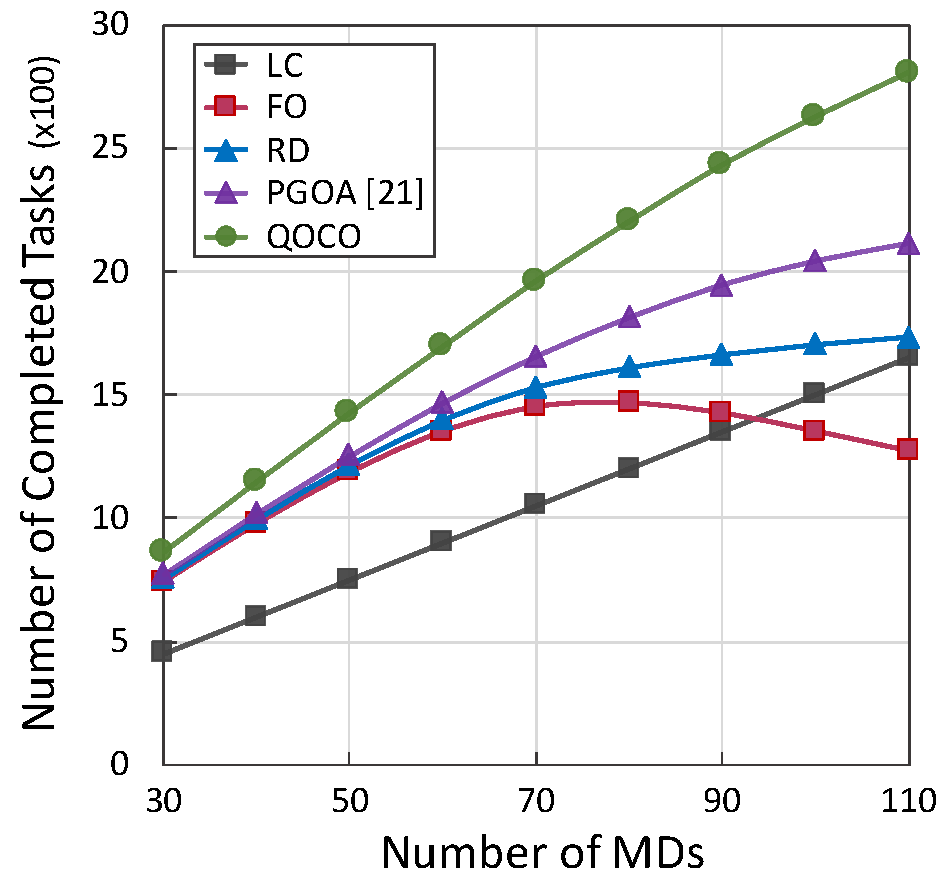
\includegraphics[width=\textwidth]{112}
       \hspace{0.6cm}(b)
	\end{minipage}

	%\caption{The number of completed tasks under different computation workloads: (a) task arrival rate; (b) the number of MDs.}
	%\label{chart1}
\end{figure}

\textcolor{teal}{Number of completed tasks} under different computation loads:
	\begin{itemize}[]
	
	\item (a) task arrival rate
	
	\item (b) the number of MDs
	
\end{itemize}
	
\end{frame}


\begin{frame}
	\frametitle{Performance Comparison}
	
	\begin{figure}
		%\captionsetup{name=Fig.}
		\begin{minipage}[b]{0.47\linewidth}
			\centering
			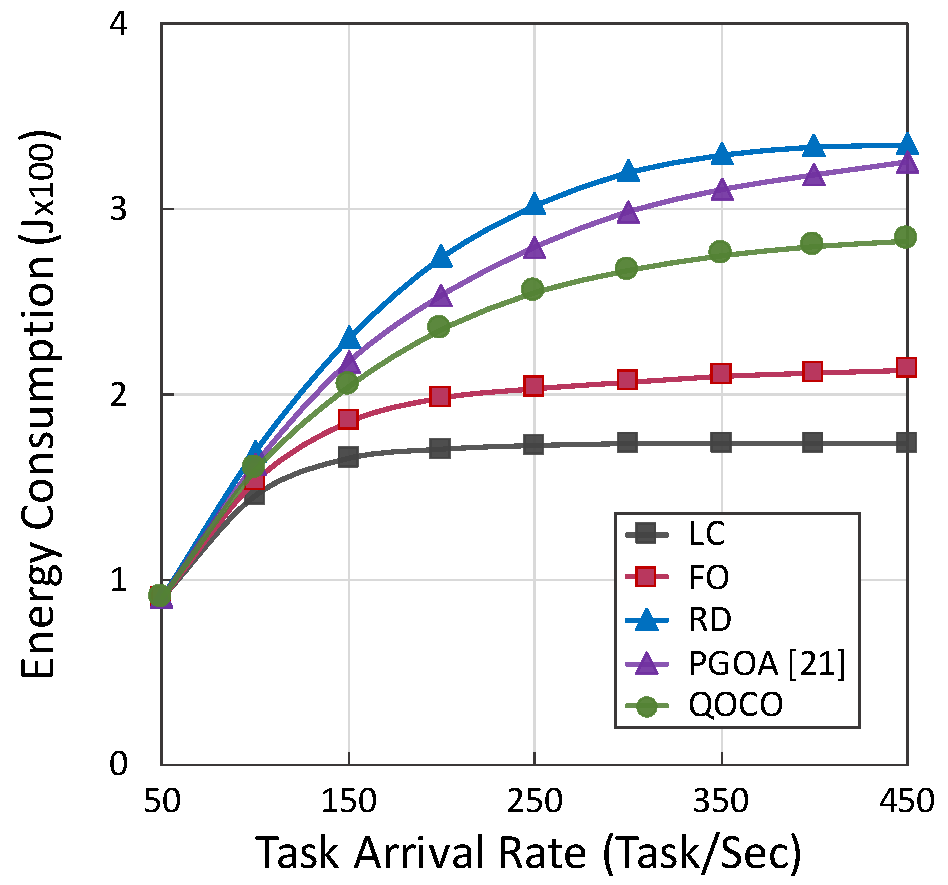
\includegraphics[width=\textwidth]{222} 
			\hspace{0.6cm}(a)
		\end{minipage}
		\hspace{-0.2cm}
		\begin{minipage}[b]{0.47\linewidth}
			\centering
			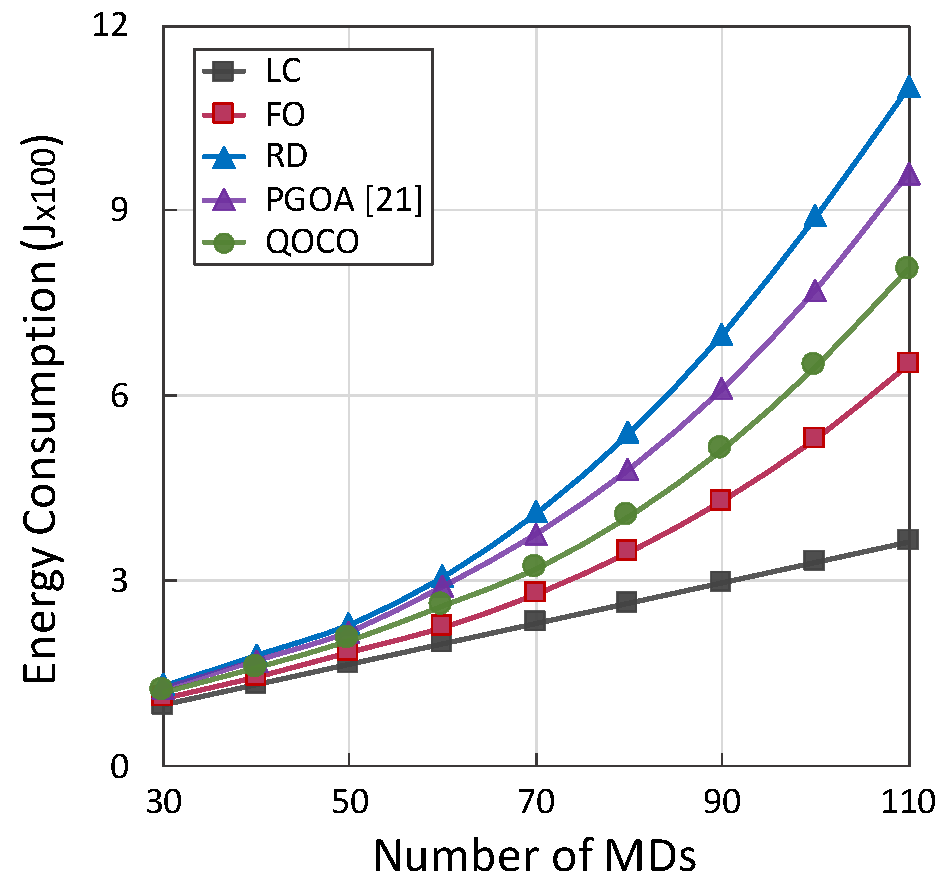
\includegraphics[width=\textwidth]{223}
			\hspace{0.6cm}(b)
		\end{minipage}
		
		%\caption{The number of completed tasks under different computation workloads: (a) task arrival rate; (b) the number of MDs.}
		%\label{chart1}
	\end{figure}
	
	\textcolor{teal}{Overall energy consumption} under different computation loads:
	\begin{itemize}[]
		
		\item (a) task arrival rate
		
		\item (b) the number of MDs
		
	\end{itemize}
	
\end{frame}


\begin{frame}
	\frametitle{Performance Comparison}
	
	\begin{figure}
		%\captionsetup{name=Fig.}
		\begin{minipage}[b]{0.47\linewidth}
			\centering
			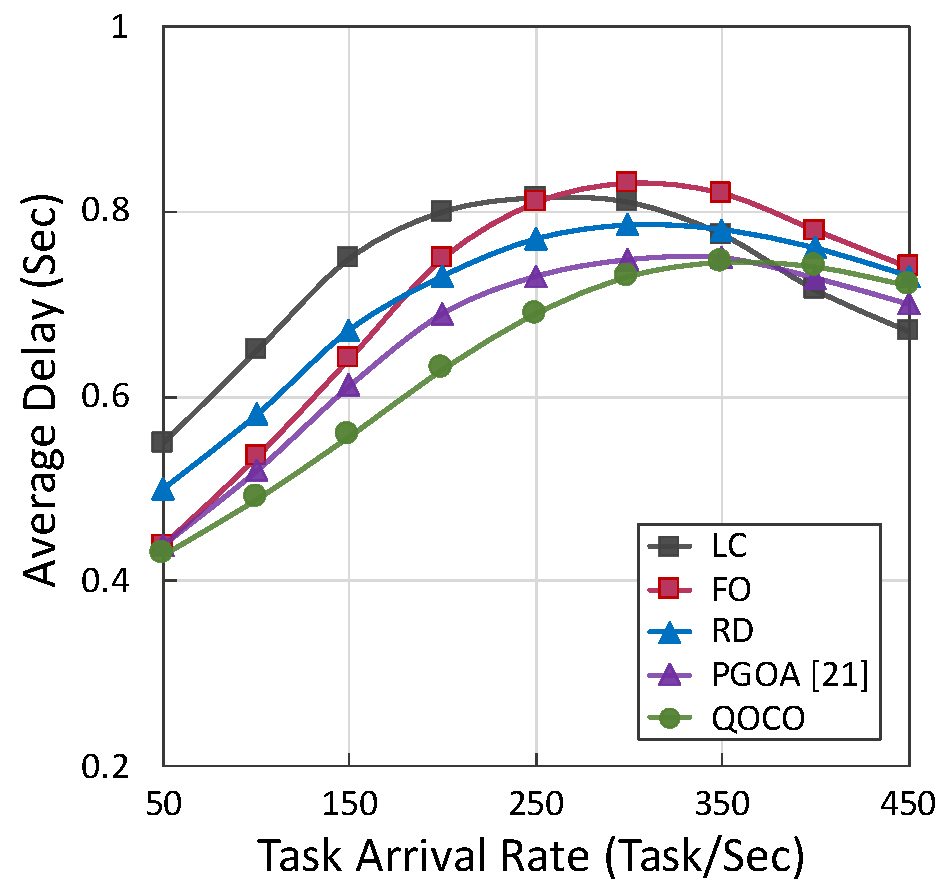
\includegraphics[width=\textwidth]{333} 
			\hspace{0.6cm}(a)
		\end{minipage}
		\hspace{-0.2cm}
		\begin{minipage}[b]{0.47\linewidth}
			\centering
			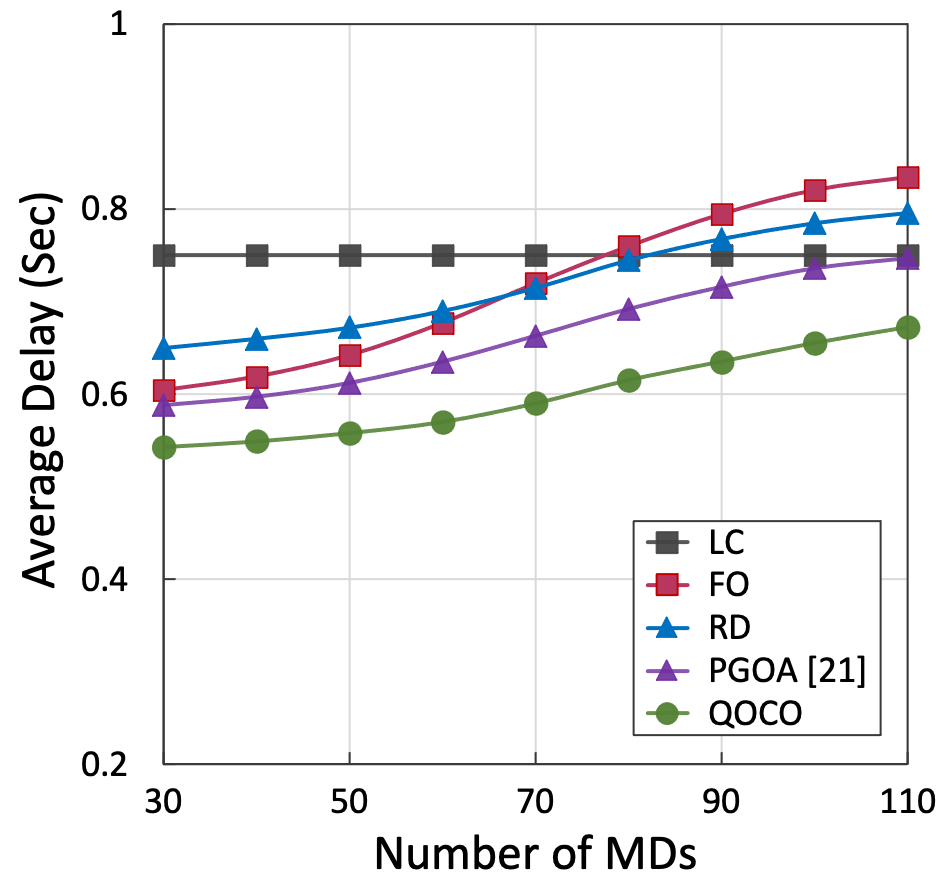
\includegraphics[width=\textwidth]{334}
			\hspace{0.6cm}(b)
		\end{minipage}
		
		%\caption{The number of completed tasks under different computation workloads: (a) task arrival rate; (b) the number of MDs.}
		%\label{chart1}
	\end{figure}
	
	\textcolor{teal}{Average delay} under different computation loads:
	\begin{itemize}[]
		
		\item (a) task arrival rate
		
		\item (b) the number of MDs
		
	\end{itemize}
	
\end{frame}


\begin{frame}
	\frametitle{Performance Comparison}
	
	\begin{figure}
		%\captionsetup{name=Fig.}
		\begin{minipage}[b]{0.47\linewidth}
			\centering
			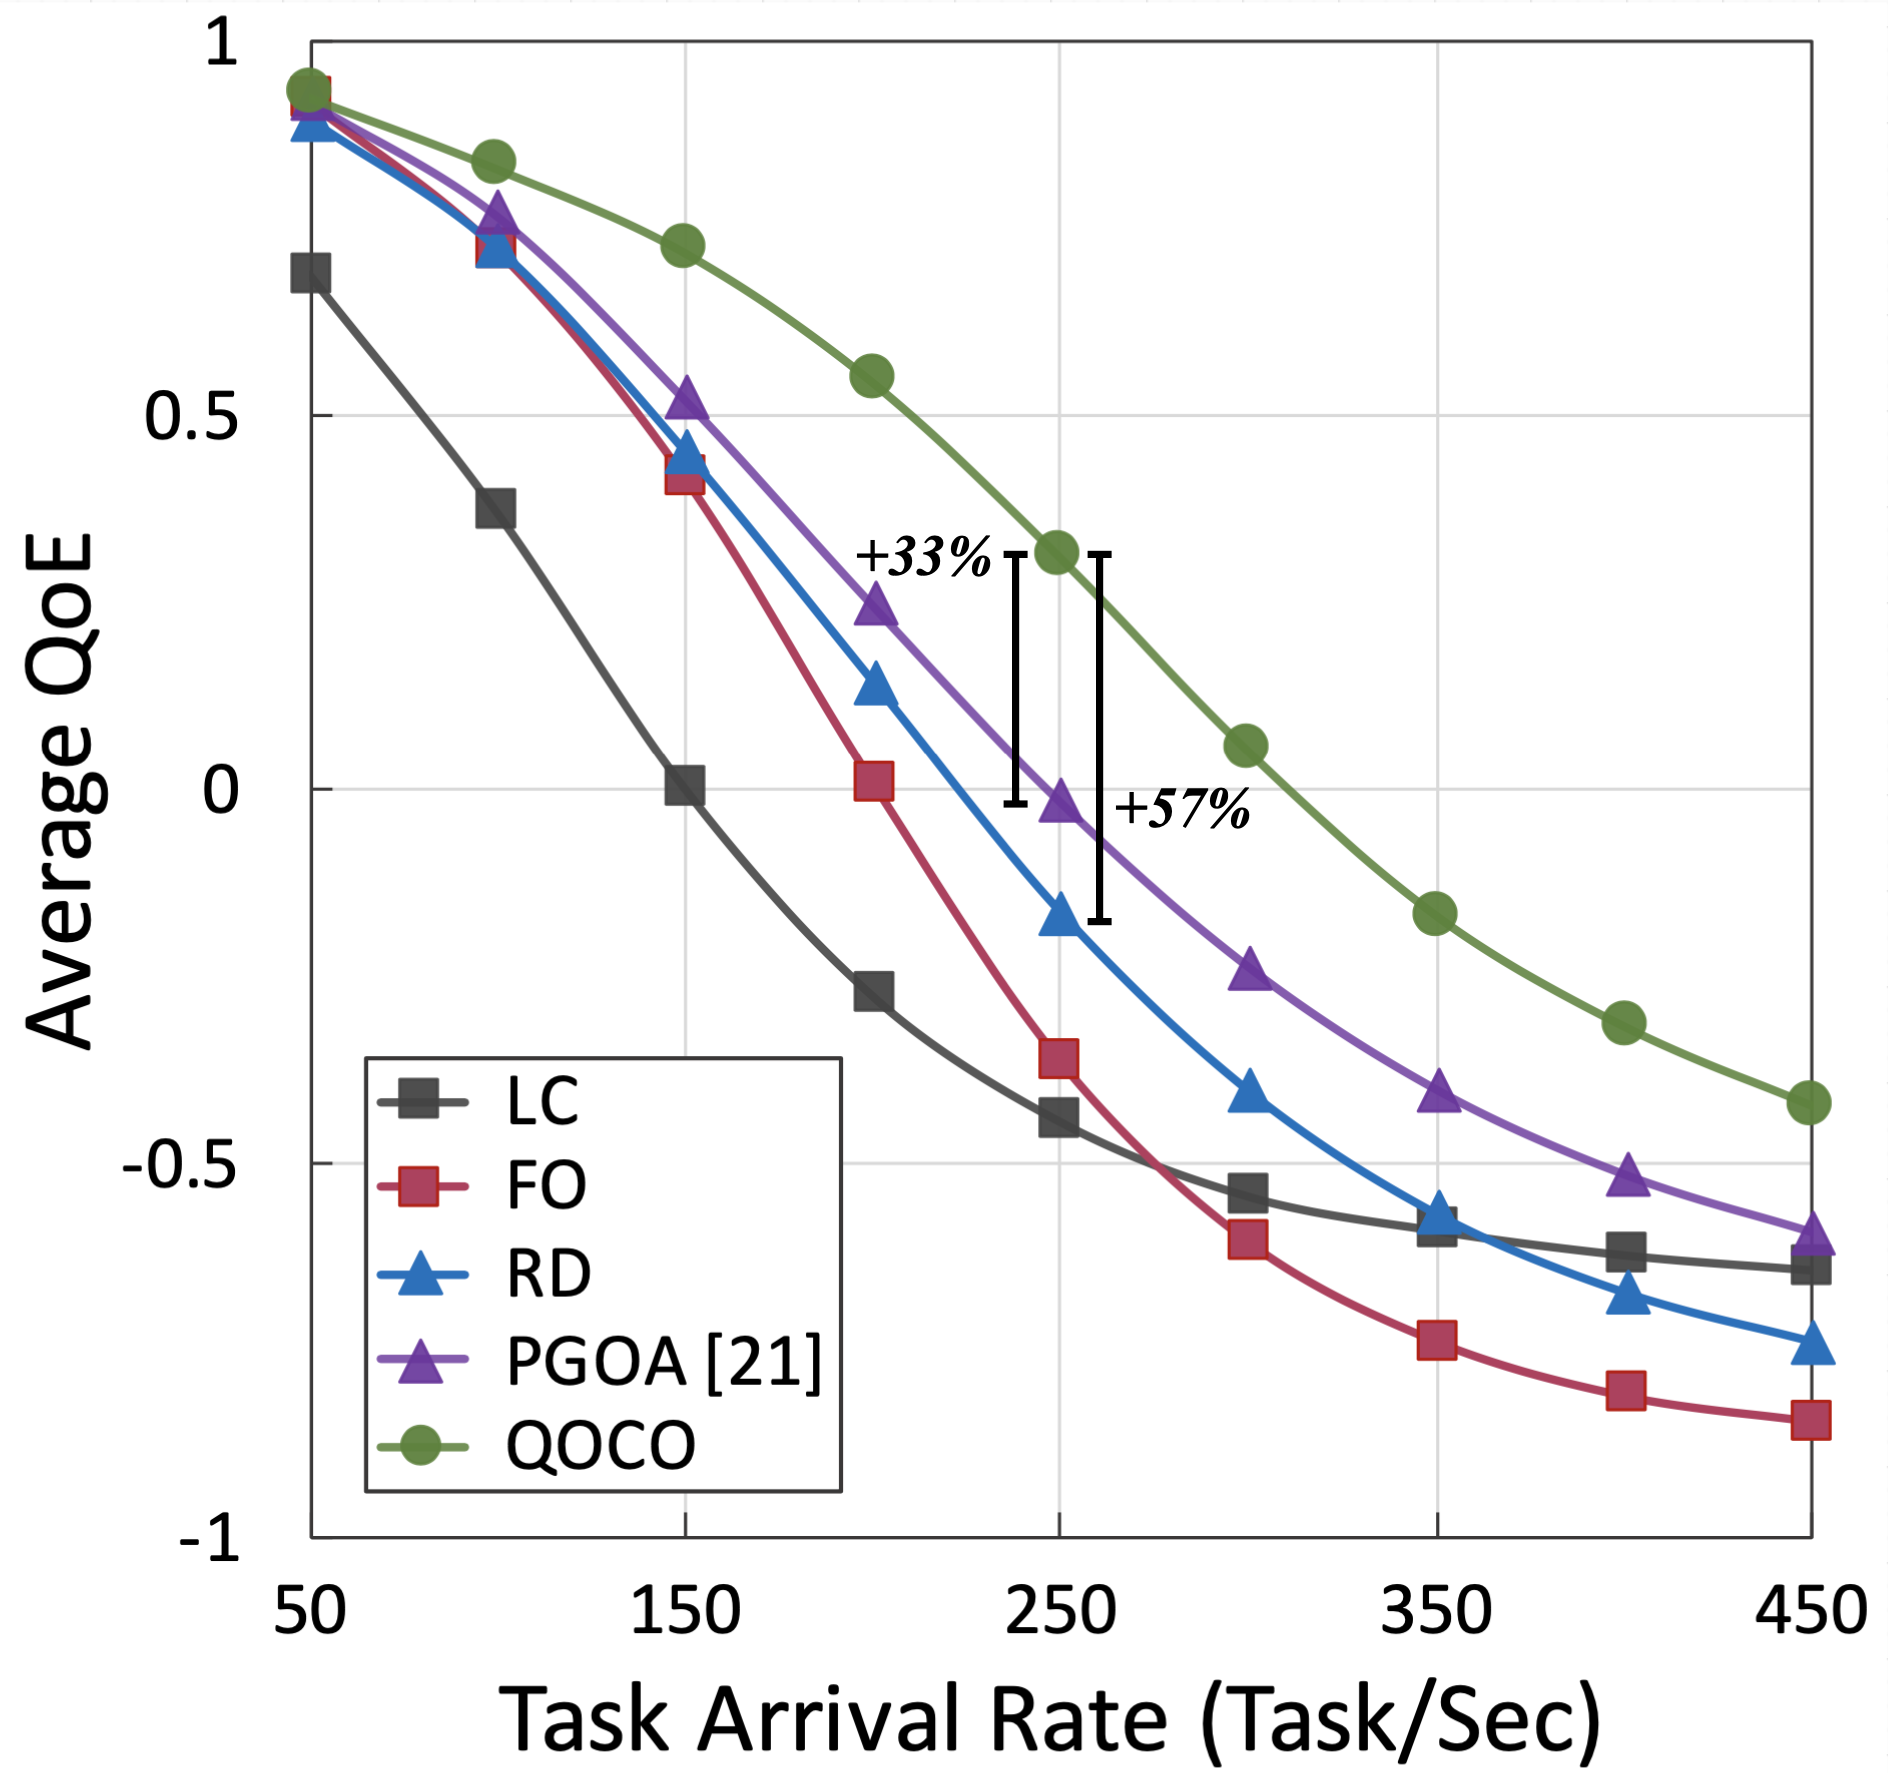
\includegraphics[width=\textwidth]{444_} 
			\hspace{0.6cm}(a)
		\end{minipage}
		\hspace{-0.2cm}
		\begin{minipage}[b]{0.47\linewidth}
			\centering
			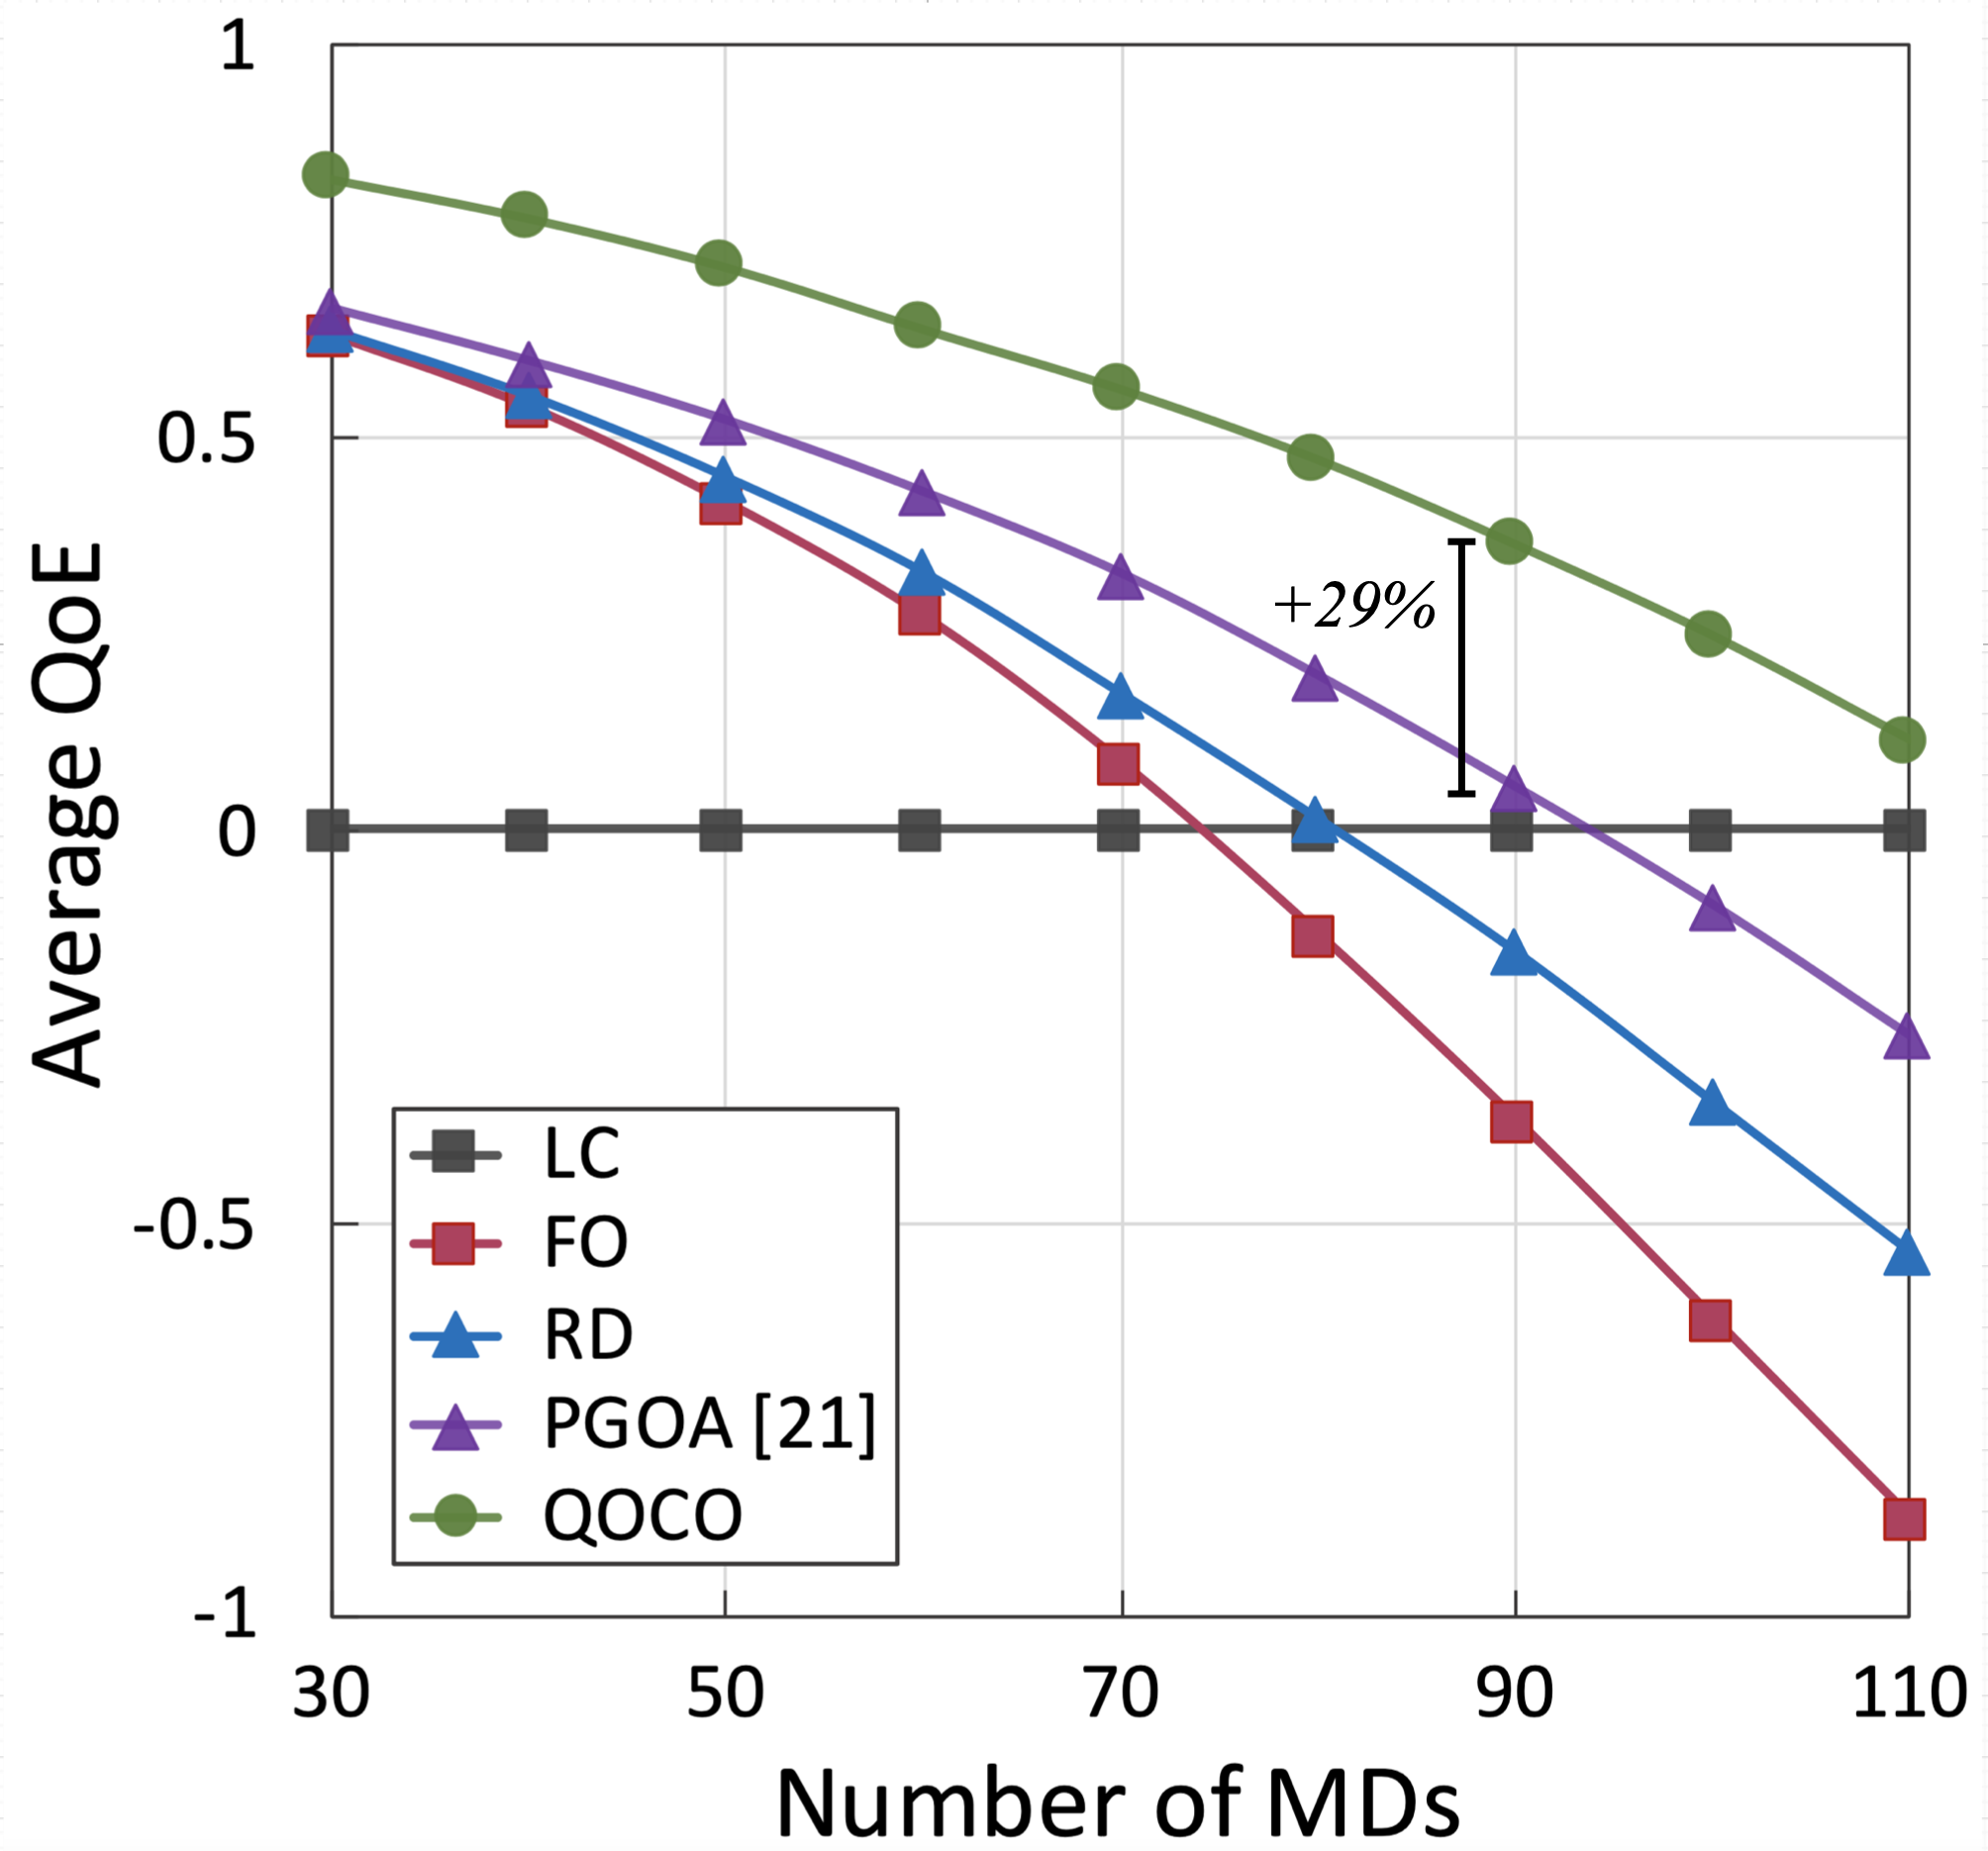
\includegraphics[width=\textwidth]{445_}
			\hspace{0.6cm}(b)
		\end{minipage}
		
		%\caption{The number of completed tasks under different computation workloads: (a) task arrival rate; (b) the number of MDs.}
		%\label{chart1}
	\end{figure}
	
	\textcolor{teal}{Average \textbf{QOE}} under different computation loads:
	\begin{itemize}[]
		
		\item (a) task arrival rate
		
		\item (b) the number of MDs
		
	\end{itemize}
	
\end{frame}



